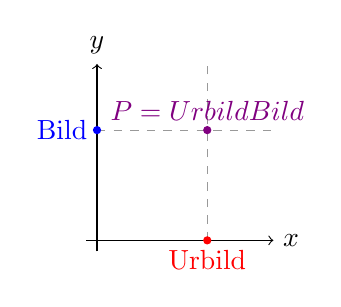
\begin{tikzpicture}[scale=0.7]
    \draw[->] (-0.2,0) -- (3.2,0) node[right] {$x$};
    \draw[->] (0,-0.2) -- (0,3.2) node[above] {$y$};
    \draw[dashed,black!40] (2,0) -- (2,3.2);
    \draw[dashed,black!40] (0,2) -- (3.2,2);
    
    \fill[red] (2,0) circle[radius=0.75mm] node[below] {Urbild};
    \fill[blue] (0,2) circle[radius=0.75mm] node[left] {Bild};
    \fill[violet] (2,2) circle[radius=0.75mm] node[above] {$P=\coord{\text{Urbild}}{\text{Bild}}$};
\end{tikzpicture}